% !TEX root=/home/tavant/these/manuscript/src/manuscript.tex

\section{Non-isothermal  fluid model }
\label{sec-fluid}

We have seen in \cref{sec-kinetic} that the polytropic law presented in \cref{eq-poly} can be used to describe the evolution of the electron temperature, hence closing the fluid equations.
Provided that the electron pressure is $p_e = e n_e \Te$, assuming the sheath collisionless, and neglecting the electron mean velocity compared to the thermal velocity, the electron momentum conservation
\begin{equation}
\label{eq-elec_mom}
 \nabla (n_e \Te) + n_e \nabla \phi = 0
\end{equation}
results in
\begin{equation}
  \label{eq-momentum}
  \nabla \Te = - \frac{\gamma - 1}{\gamma} \nabla \phi
\end{equation}
Integrating \cref{eq-elec_mom} from the sheath edge, the electron density is hence:
\begin{equation}
  \label{eq-ne}
  n_e(\phi) = n_0 \left[ 1 + \frac{(\gamma - 1) (\phi - \phi_0)}{\gamma \Te_0}  \right]^{\frac{1}{\gamma - 1}}
\end{equation}
with the subscript $0$ corresponds to the sheath edge.
In \cref{eq-ne}, we need to have $\gamma$ strictly greater than one.
For $\gamma=1$, we find the usual Boltzmann electrons:
\begin{equation}
  n_e(\phi) = n_0 \exp( - \frac{ (\phi - \phi_0)}{\Te})
\end{equation}
corresponding to the usual isothermal model.

\subsection{Comparison with the PIC simulations}
\label{sec-fluidPIC}
The PIC simulations of \cref{sec-1DPIC} can be modeled using a 1D low pressure fluid model with collisionless ions.
We use the solver described in \citet{riemann2005}, modified to take into account the new electron closure.
We simply need to add one equation for the temperature, and the ionization source term is fixed constant in space.

Using the normalized variables and parameters:
\begin{align}
\lambda &= \frac{S_{iz} L}{c_s}, &\Phi&=-\frac{e \phi}{\Te_{, c}}, &u &= \frac{v_i}{c_s}\\
n &= \frac{n_i}{n_{e,c}}, &\chi&=\lambda \frac{x}{L}, &\epsilon &= \lambda \frac{\lambda_{De}}{L}\\
\end{align}
with $\Te_{,c}, n_{e,c}$ the electron temperature and density at the center, $c_s= \sqrt{\frac{\Te_{,c}}{m_i}}$ the ion sound speed, $v_i, n_i$ the ion speed and density, and $S_{iz}$ the ionization frequency, we can write the set of equations representing the plasma as\citep{riemann2005}:



\begin{equation}
  \label{eqs-fluid}
  \begin{cases}
    d_{\chi} (n u ) &= \lambda\\
    d_{\chi} (u) &= \frac{d_{\chi} (\phi)}{u} - \frac{\lambda}{n}\\
    d_{\chi}^2 (\Phi) &= \frac{(n - n_e)}{\epsilon^2}\\
    S_{iz} &= cst \\
    n_{e} &= \left[ 1 + \frac{(\gamma - 1) \Phi }{\gamma}  \right]^{\frac{1}{\gamma - 1}}
\end{cases}
\end{equation}

Starting from the center, and using the results of the PIC simulations to determine $\gamma$, we can use the system of \cref{eqs-fluid} to compute the profile of every variable.
The plasma potential is self consistently computed from an arbitrary value at the center.
It is then shifted to set the wall potential to 0V.
The integration uses the \nth{4} order Runge-Kutta integration scheme of the python package \texttt{scipy}.


\begin{figure}[!htbp]
  \centering
  % 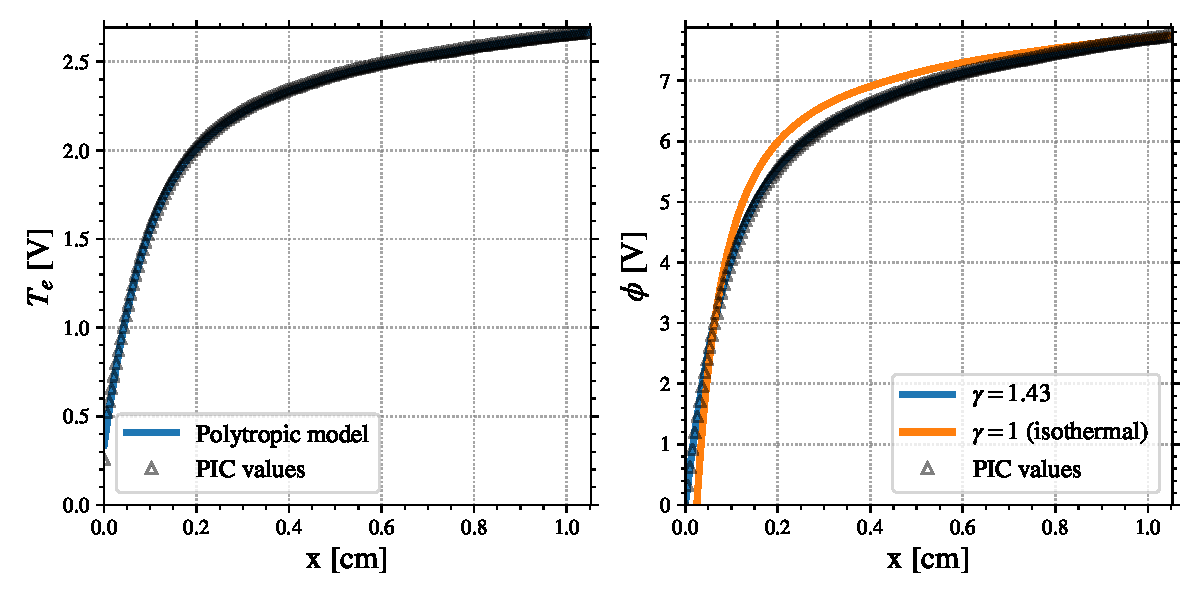
\includegraphics[width = 0.7\textwidth]{figures/sheathModel.pdf}
  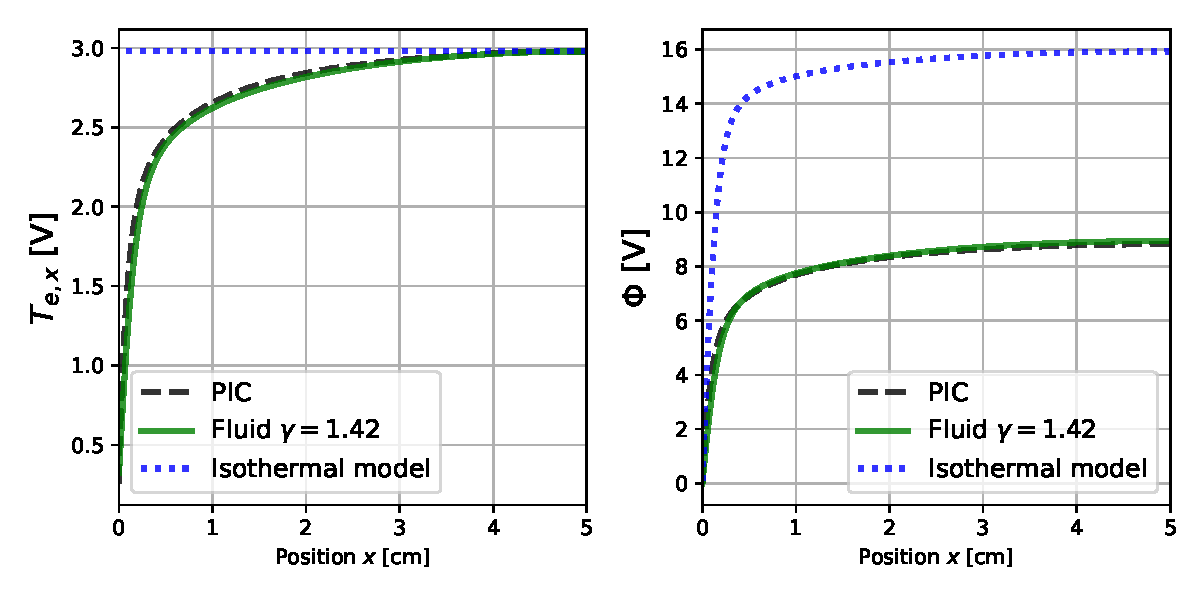
\includegraphics[width = 0.9\textwidth]{FluidComparison.pdf}
  \caption{Comparison of the electron temperature and plasma potential measured in the PIC simulation with the prediction of the polytropic model with $\gamma = 1.42$.}
  \label{fig-comp}
\end{figure}

\Cref{fig-comp} shows the comparison of the electron temperature and the plasma potential with the resolution of the set of \cref{eqs-fluid}.
We can see a very good agreement between the model and the PIC simulations.


\subsection{Modified Bohm criterion}
The Bohm criterion expresses a necessary condition on the ion velocity at the sheath edge for the formation of a stationary sheath \citep{riemann1991}.
As discussed in the appendix, it is possible to derive a modified Bohm criterion for the polytropic electrons:
\begin{equation}
  \mathcal{M}^2 = \left( \frac{u_0}{c_s} \right)^2 \geq \gamma
\end{equation}
with $\mathcal{M}$ the Mach number, $u_0$ the ion mean velocity at the sheath edge and $c_s=\left( \frac{e \Te_0}{m_i} \right)^{1/2}$ the ion acoustic velocity at the sheath edge. The derivation of this modified Bohm criterion is analogous to the isothermal case.
In the same way as for the isothermal Debye sheath, we assume that the sheath criterion is saturated:
\begin{equation}
  \label{eq-saturation}
  \mathcal{M}^2 = \gamma.
\end{equation}

In addition, the ion flux at the wall is equal to the flux at the sheath edge:
\begin{equation}
  \label{eq-gi}
  \Gamma_i = n_0 \sqrt{\frac{\gamma e \Te_0}{m_i}}
\end{equation}

\subsection{Plasma potential drop to the wall}
The electron flux at the wall is the thermal flux:
\begin{equation}
  \label{eq-geki}
  \Gamma_e = \int_0^{+\infty} v f_e(x=x_w,v) dv
\end{equation}
Using the model of two-Te EEDF described in \ref{sec-twoTe}, we obtain
\begin{equation}
  \label{eq-ge}
  \Gamma_e = \frac{1}{4} n_{e,w} \bar{v}_w
\end{equation}
with $n_{e,w}$ the electron density at the wall, and $\bar{v}_w = \sqrt{\frac{8 e\Te_{,w}}{\pi m_e}}$ the mean electron speed at the wall, using $\Te_{,w}$ the electron temperature at the wall.
Using \cref{eq-momentum}, we have:
\begin{equation}
  \label{eq-tew}
  \Te_{,w} = \Te_0 \left(  1 - \frac{\gamma -1}{\gamma}\frac{\dphi_0}{\Te_0}  \right)
\end{equation}
with $\dphi_0$ the potential drop between the sheath edge and the wall.
Using the current equality: $\Gamma_i = \Gamma_e$ at the wall we find with \cref{eq-gi,eq-ge,eq-tew}:
\begin{equation}\label{eq-sheath}
  \left[ 1 +\frac{\gamma -1}{\gamma} \frac{ \dphi_0}{ \Te_0}  \right]^{\frac{1}{\gamma - 1}} \sqrt{1 - \frac{\gamma -1}{\gamma}\frac{\dphi_0}{\Te_0}} = \sqrt{\frac{4 \gamma \pi m_e}{m_i}}
\end{equation}

\Cref{eq-sheath} cannot be solved analytically, but it can be solved numerically.
We use the function \texttt{fsolve} from python package \texttt{scipy.optimize} to plot the solution of \cref{eq-sheath} in \cref{fig-dphinorm}.
Meanwhile, we estimate $\frac{\Delta \phi_0}{\Te_0}$ using the fluid model of \cref{sec-fluid} by reading the potential at the position for which the ions reach the modified Bohm velocity.
The small difference between the solution of \cref{eq-sheath} and the fluid solution is due to the presence of ionization in the sheath.

\begin{figure}[!htbp]
  \centering
  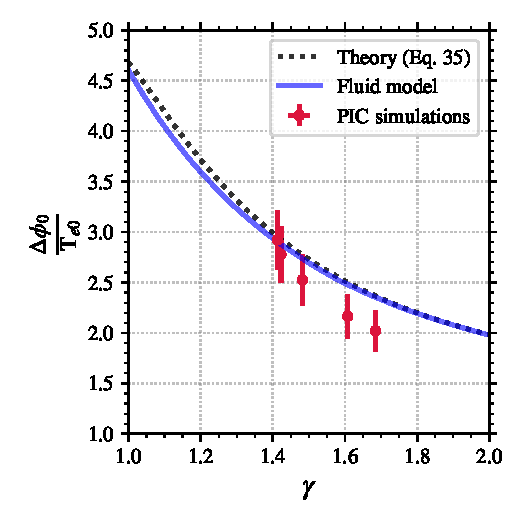
\includegraphics[width=\defaultwidth]{phinorm_theoryAndPIC2.pdf}
  \caption{Evolution of the potential drop normalized to the electron temperature as a function of the polytropic index $\gamma$ from the theory of \cref{eq-sheath}, from the fluid model of \cref{sec-fluidPIC} and from the PIC simulations results (the same cases as in \cref{fig-p}). Errors correspond to 10\% . }
  \label{fig-dphinorm}
\end{figure}


\Cref{fig-dphinorm} shows the evolution of normalized plasma potential drop to the wall $\frac{\dphi_0}{\Te_0}$ as a function of $\gamma$.
{  Error bars indicate an uncertainty of 10\%.
This uncertainty value corresponds to an aggregation of the numerical fluctuation of the PIC simulation (that decreases when more particles per cell are used), and the estimation of the sheath edge position.
A more accurate estimation of these uncertainties would require a dedicated study with many additional simulations, hence we choose the reasonable value of 10\% \citep{turner2013}.}
We can see that in the limit where $\gamma \rightarrow 1$, we find with \cref{eq-sheath} the usual isothermal value $\frac{\dphi_0}{\Te_0}  \simeq 4.68$ for argon.
The value observed in the fluid model is very close to the results of \cref{eq-sheath}.
This is due to the very small size of the sheath, as seen in \cref{fig-PIC1}.
When $\gamma$ increases, $\frac{\dphi_0}{\Te_0}$ decreases significantly.
The decrease of $\dphi_0$ is consistent with the depletion of the high energy tail of the electrons, as the plasma needs less screening of the electrons in order to stay quasi-neutral.

\Cref{fig-dphinorm} also presents the potential drop measured in the same PIC simulations as presented in \cref{fig-p}.
The error bars correspond to an estimate of the aggregation of the uncertainties from the PIC simulation and the averages.
The sheath edge is defined using the modified Bohm criterion (\cref{eq-saturation}), as for the fluid model.
We can see a very good agreement with the theories.
The trend of decreasing potential drop with increasing $\gamma$ is clearly observed, and the values agree within about $10\%$.
This is significantly more accurate than the $50$\% discrepancy with respect to the isothermal model.

The solutions of \cref{eq-sheath} can be fitted between $\gamma = 1$ and $\gamma = 2$ with a good precision ($R^2 = 0.98$) by:
\begin{equation}
  \label{eq-fit}
  \frac{\dphi_0}{\Te_0} = 0.7 + \frac{4.1}{\gamma^{1.7}}
\end{equation}
%Although the expression of \cref{eq-fit} has no physical origin.

\subsection{Power losses at the wall}

As expressed in the previous section, the electron flux to the wall is equal to the ion flux:
\begin{equation}
  \Gamma_e = \Gamma_i =  n_0 \sqrt{\frac{\gamma e \Te_0}{m_i}}
\end{equation}
with $n_{e,0}$ and $\Te_0$ the electron density and temperature at the sheath edge.
Following the two-$\Te$ EEDF as described in \cref{sec-kinetic}, the electron energy flux to the wall is a thermal flux from a Maxwellian distribution function of temperature  $\Te_w$.
Hence it reads \cite{chabert2011}:
\begin{equation}
  \label{eq-maxflux}
  Q_e = \Gamma_e 2 \Te_{w}
\end{equation}

Using \cref{eq-tew}, we obtain
\begin{equation}
  \label{eq-meanE}
  \frac{Q_e}{\Gamma_e} =  2 \Te_0 \left[1 - \frac{(\gamma - 1)}{\gamma} \frac{\dphi_0}{\Te_0} \right]
\end{equation}
with $\frac{\dphi_0}{\Te_0}$ calculated from either \cref{eq-sheath} or \cref{eq-fit}.
From \cref{eq-meanE} we see that in the isothermal limit we find the usual $2 \Te$ mean energy by electron leaving the plasma.
However, for $\gamma > 1$, the mean energy by electron decreases.


\begin{figure}[!htbp]
  \centering
  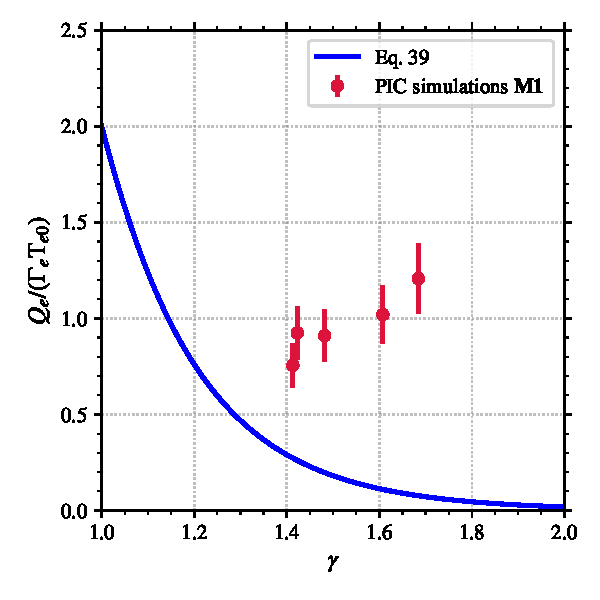
\includegraphics[width=\defaultwidth]{meanelectronenergy_PIC.pdf}
  \caption{Evolution of the mean energy per electron leaving the plasma at the wall normalized to the electron temperature at the sheath edge as a function of the polytropic index $\gamma$ from the theory of \cref{eq-meanE}. The simulation result (marker) corresponds to the model \M1. }
  \label{fig-avE}
\end{figure}

\Cref{fig-avE} shows the evolution of the average energy of electrons leaving the plasma at the wall normalized to the electron temperature in the plasma bulk from \cref{eq-meanE}.
We can see that the ratio is significantly lower than the isothermal value $\frac{Q_e}{\Gamma_e} = 2 \Te_0$ when $\gamma > 1$.
Overlaid in \cref{fig-avE} are the PIC simulation results.
We can see that the PIC results are lower than the isothermal value, but do not agree well with \cref{eq-meanE}.
The discrepancy could be due to the two-Te hypothesis used in \cref{eq-maxflux}.
Indeed, we can see in \cref{fig-EVDFpm} that there is a small population of high energy electrons.
This population is not big enough to modify the electron flux to the wall, hence the potential drop \citep{demidov2005}, but may increase the mean energy of electron leaving the plasma.
{  We tested the hypothesis for one case ($P_n=2$ mTorr).
Once the steady state was reached, we stopped generating the electron-ion couples.
We observed that during a transition time of around $0.74 \mu$s, the mean energy per electron decreased significantly from $0.9$~V to $0.3$~V, while the electron flux to the wall $\Gamma_e$ and the electron temperature $\Te_{, 0}$ was not yet affected.
This is more consistent with \cref{eq-meanE} and seems to confirm the hypothesis, but more investigations on the heat flux are needed.
  }
